%%%%%%%%%%%%%%%%%%%%%%%%%%%%%%%%%%%%%%%%%
% Short Sectioned Assignment
% LaTeX Template
% Version 1.0 (5/5/12)
%
% This template has been downloaded from:
% http://www.LaTeXTemplates.com
%
% Original author:
% Frits Wenneker (http://www.howtotex.com)
%
% License:
% CC BY-NC-SA 3.0 (http://creativecommons.org/licenses/by-nc-sa/3.0/)
%
%%%%%%%%%%%%%%%%%%%%%%%%%%%%%%%%%%%%%%%%%

%----------------------------------------------------------------------------------------
%	PACKAGES AND OTHER DOCUMENT CONFIGURATIONS
%----------------------------------------------------------------------------------------

\documentclass[paper=a4, fontsize=11pt]{article} % A4 paper and 11pt font size

\usepackage[T1]{fontenc} % Use 8-bit encoding that has 256 glyphs
%\usepackage{fourier} % Use the Adobe Utopia font for the document - comment this line to return to the LaTeX default
\usepackage[english]{babel} % English language/hyphenation
\usepackage{amsmath,amsfonts,amsthm} % Math packages

\usepackage{sectsty} % Allows customizing section commands
\allsectionsfont{\centering \normalfont\scshape} % Make all sections centered, the default font and small caps

\usepackage{fancyhdr} % Custom headers and footers
\pagestyle{fancyplain} % Makes all pages in the document conform to the custom headers and footers
\fancyhead{} % No page header - if you want one, create it in the same way as the footers below
\fancyfoot[L]{} % Empty left footer
\fancyfoot[C]{} % Empty center footer
\fancyfoot[R]{\thepage} % Page numbering for right footer
\renewcommand{\headrulewidth}{0pt} % Remove header underlines
\renewcommand{\footrulewidth}{0pt} % Remove footer underlines
\setlength{\headheight}{13.6pt} % Customize the height of the header

\numberwithin{equation}{section} % Number equations within sections (i.e. 1.1, 1.2, 2.1, 2.2 instead of 1, 2, 3, 4)
\numberwithin{figure}{section} % Number figures within sections (i.e. 1.1, 1.2, 2.1, 2.2 instead of 1, 2, 3, 4)
\numberwithin{table}{section} % Number tables within sections (i.e. 1.1, 1.2, 2.1, 2.2 instead of 1, 2, 3, 4)

\setlength\parindent{0pt} % Removes all indentation from paragraphs - comment this line for an assignment with lots of text

\usepackage{hyperref}
\usepackage{geometry}
 \geometry{
 a4paper,
 left=12mm,
 right=12mm,
 top=12mm,
 bottom=20mm,
 }
\usepackage{graphicx}
\usepackage{multirow}
\usepackage{wrapfig}

%----------------------------------------------------------------------------------------
%	TITLE SECTION
%----------------------------------------------------------------------------------------

\begin{document}

\title{Charlie's notes}

\maketitle
%----------------------------------------------------------------------------------------
%	PROBLEM 1
%----------------------------------------------------------------------------------------

\section{CS31310 - Agile}




%------------------------------------------------

\section{CS36110 - Machine Learning}


%------------------------------------------------

\section{CS34110 - Computer Vision}

\subsection{November 20: Motion Models}

\textbf{Modelling Change \& Tracking}

\paragraph{Motion:}
\begin{itemize}
\item Background Subtraction
\item Optical Flow
\end{itemize}

\paragraph{Mixture of Gaussians (MoG):}
\begin{itemize}
\item Robust to noise
\item Handles shadows ok
\item Common first step
\end{itemize}

\subsubsection{Tracking: Modelling change}

\paragraph{Video:}
\begin{itemize}
\item detections in each frame
\item detections are noisy \& computationally expensive
\item tracking mitigates both issues
\end{itemize}

Noise can occur if the camera on a robot/car is moving up/down

\subsubsection{A general framework for tracking}

\paragraph{Recursively:}
\begin{itemize}
\item An idea about how something will change (\textit{Model})
\item Make a prediction (\textit{Predict})
\item See what happens (\textit{Measure})
\item Update model (\textit{Update})
\end{itemize}

\paragraph{Advantages:}
\begin{itemize}
\item Smooths the data 
	\begin{itemize}
	\item	estimate location upon predictions  \& the measurement
	\end{itemize}
\item Constrains search
	\begin{itemize}
	\item start looking for target in the location it was last seen		
	\end{itemize}
\end{itemize}

\subsubsection{Kalman Filter}

\begin{itemize}
\item Like predict, measure, update from earlier
\item Useful for tracking
\item Copes well with missing information (occlusions) 
\end{itemize}

\begin{figure}[h]
    \centering
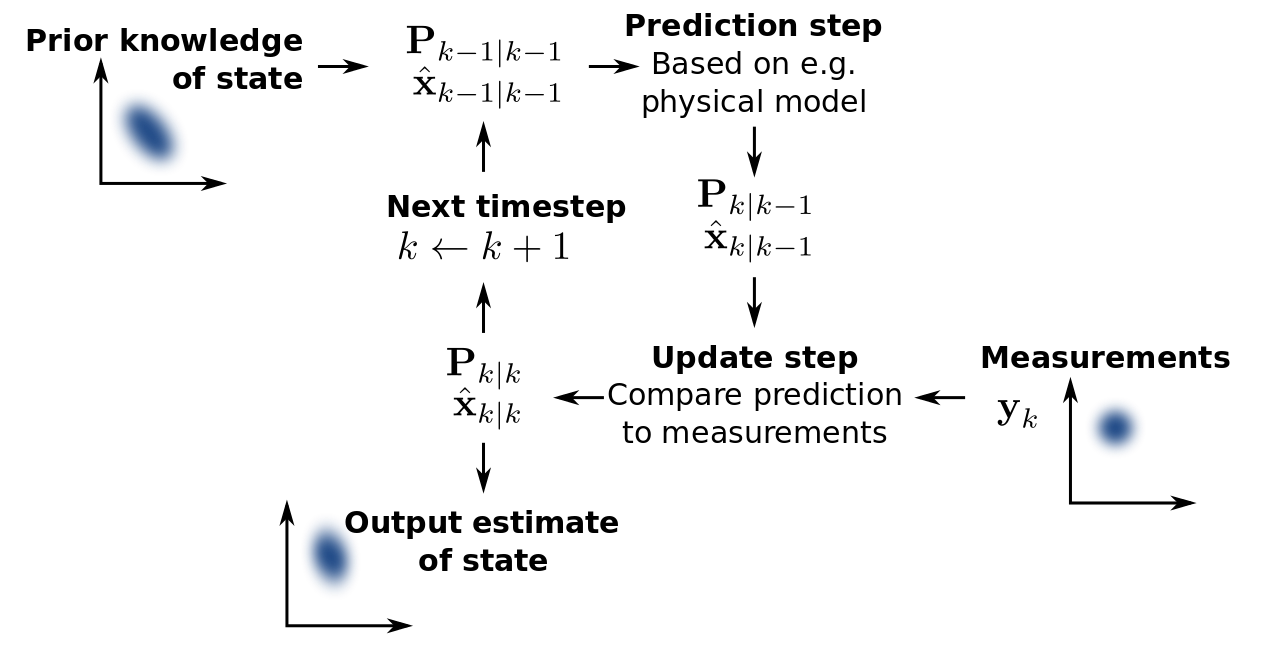
\includegraphics[scale=0.3]{images/kalman}
\caption{Sourced from Wikipedia}
    \label{fig:kalman}
\end{figure}

\begin{center}

\begin{tabular}{| c  c  c  c | c |}
\hline
Background subtraction & $\rightarrow$ & Pixels grouped into objects & $\rightarrow$ & \multirow{3}{4em}{Tracker} \\ 
Sparse Optical Flow &  $\rightarrow$  & Features grouped into objects &  $\rightarrow$  & \\ 
Face Detection &   $\rightarrow$   &  $\rightarrow$  &   $\rightarrow$   & \\ \hline

\end{tabular}
\end{center}

\paragraph{Use Kalman to smooth any measurement}
\begin{itemize}
\item X,Y location
\item size
\item colour
\end{itemize}

\textbf{See also:} Particle filtering: works with combining and splitting objects (e.g. people holding hands, then letting go)

\textbf{Hannah's video: } \url{https://www.youtube.com/watch?v=NYdwpX1a7-Y}

\subsubsection{Mean Shift}

\begin{wrapfigure}{r}{0.5\textwidth}
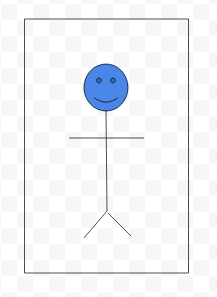
\includegraphics[scale = 0.5]{images/mean_shift}
\end{wrapfigure}

Computer the mean of the data within the window

Shift the window to the mean every time

\paragraph{Notes:}
\begin{itemize}
\item Changes size - can use CAM-Shift to mitigate?
\item Lighting change - not really, gradually changes mean over time
\item If it picks up something you're not looking for, will slowly drift off
\end{itemize}

\subsubsection{Problems with Tracking}

\begin{itemize}
\item Initialisation (what are you tracking?)
\item Having more than 1 item to track
\item Losing target due to motion / occlusion
\item Losing target due to appearance change
\end{itemize}

Usually initialise from a detector of some sort

\textbf{Useful speed up for detectors \& accuracy}

Look into: TLD: Tracking Learning Description

\subsubsection{Closing note}

Vision Systems tend to have multiple layers

Tracking is extremely common in anything which deals with change.

\paragraph{HOG for example, has several layers:}
\begin{itemize}
\item 2D filters
\item Tangent
\item Histogram
\item Superimpose grid
\item SVM
\end{itemize}
\textit{May be more, however couldn't write quick enough... You get the idea...}

\rule{\textwidth}{1pt}

%-------------------------------------------------

\section{CS32310 - Advanced Computer Graphics}

%------------------------------------------------

\section{SE31520 - Internet-based Applications}


%------------------------------------------------

\section{Other}

%----------------------------------------------------------------------------------------

\end{document}